
% This LaTeX was auto-generated from an M-file by MATLAB.
% To make changes, update the M-file and republish this document.

\documentclass{article}
\usepackage{amsmath,amsfonts,amsthm,amssymb}
\usepackage{fullpage,fancyhdr}
\usepackage[pdftex]{graphicx}
\usepackage[usenames,dvipsnames]{color}
\usepackage{listings}
\usepackage{courier}
\usepackage{ifthen}
\usepackage{setspace}
\usepackage{lastpage}
\usepackage{extramarks}
\usepackage{chngpage}
\usepackage{soul}
\usepackage{graphicx,float,wrapfig}
\usepackage{epstopdf}
\usepackage{geometry}
\usepackage{pdfcolmk}
\usepackage{hyperref}
\DeclareGraphicsRule{.tif}{png}{.png}{`convert #1 `dirname #1`/`basename #1 .tif`.png}

\definecolor{lightgray}{gray}{0.5}
\definecolor{darkgray}{gray}{0.3}
\definecolor{MyDarkGreen}{rgb}{0.0,0.4,0.0}

\topmargin=-0.45in      %
\evensidemargin=0in     %
\oddsidemargin=0in      %
\textwidth=6.5in        %
\textheight=9.0in       %
\headsep=0.25in         %

\pagestyle{fancyplain}
 
\fancyhf{}
 
\lhead{\fancyplain{}{Michael Carroll}}
\chead{\fancyplain{}{ELEC6230 - Parallel Processing}}
\rhead{\fancyplain{}{\today}}
\rfoot{\fancyplain{}{\thepage\ of \pageref{LastPage}}}

\sloppy
\setlength{\parindent}{0pt}

\lstloadlanguages{C++}
\lstset{
language=C++,
frame=single,
basicstyle=\ttfamily,
keywordstyle=[1]\color{Blue}\bf,
keywordstyle=[2]\color{Purple},
keywordstyle=[3]\color{Blue}\underbar,
identifierstyle=,
numbers=left,
numberstyle=\tiny\color{Blue},
stepnumber=5,
morekeywords={printf,atoi,omp,parallel,shared,schedule,reduction},
morekeywords=[2]{gettimeofday,matrixSize,omp_get_wtime,omp_set_num_threads}
}

% Alter some LaTeX defaults for better treatment of figures:
% See p.105 of "TeX Unbound" for suggested values.
% See pp. 199-200 of Lamport's "LaTeX" book for details.
%   General parameters, for ALL pages:
\renewcommand{\topfraction}{0.9}	% max fraction of floats at top
\renewcommand{\bottomfraction}{0.8}	% max fraction of floats at bottom
%   Parameters for TEXT pages (not float pages):
\setcounter{topnumber}{2}
\setcounter{bottomnumber}{2}
\setcounter{totalnumber}{4}     % 2 may work better
\setcounter{dbltopnumber}{2}    % for 2-column pages
\renewcommand{\dbltopfraction}{0.9}	% fit big float above 2-col. text
\renewcommand{\textfraction}{0.07}	% allow minimal text w. figs
%   Parameters for FLOAT pages (not text pages):
\renewcommand{\floatpagefraction}{0.7}	% require fuller float pages
% N.B.: floatpagefraction MUST be less than topfraction !!
\renewcommand{\dblfloatpagefraction}{0.7}	% require fuller float pages

% remember to use [htp] or [htpb] for placement

\title{ELEC6230 Homework 5\\
{\large \begin{par}
Answers to Parallel Processing Homework 5
\end{par} \vspace{1em}
}}
\author{Michael J. Carroll}

\begin{document}
\maketitle

\section*{Question 1 Results}
\begin{par}
I created the sequential C++ program included below in Appendix A.

The execution time are detailed in the following table:
\end{par}

\begin{table}[tbph]
\begin{center}
\begin{tabular}[tbph]{| l | r |}
\hline
Total Execution Time & 110.277 Seconds \\
Setup Time & 0.086 Seconds \\
Multiplication Time & 110.177 Seconds \\
Error (C vs C expected) & 0 \\
\hline
\end{tabular}
\caption{Execution Time in Seconds for 1 PE, Sequential}
\end{center}
\end{table}

\section*{Question 2 Results}
\begin{par}
I created the parallel (OpenMP) C++ program included below in Appendix B.  I opted to use static scheduling, and varied the chunk size to see what effect that the size had on the execution time.  I determined that a chunk size of 10 gives the best results for this program.\\
The program execution time is primarily a function of the matrix multiplication time, so parallelizing that has the largest effect on the execution time.  One thing that is interesting is that using 5 PEs is actually more efficient than using 6 PEs.  This could be due to some unknown overhead in the program.
\end{par}

\begin{table}[tbph]
\begin{center}
\begin{tabular}[tbph]{| l | r | r | r | r | r | r |}
\hline
Number of PEs & 1 & 2 & 3 & 4 & 5 & 6 \\
\hline
Total Execution Time & 111.5312 & 59.1370 & 39.7929 & 30.6846 & 24.0189 & 21.7737 \\
Matrix Creation Time & 0.1012 & 0.0618 & 0.0412 & 0.0702 & 0.0430 & 0.0997 \\
Multiplication Time & 111.4125 & 59.0664 & 39.7455 &  30.6097 &  23.9722 & 21.6710 \\
Error Checking Time & 0.0174 & 0.0088 & 0.0061& 0.0046 & 0.0037 & 0.0030 \\
\hline
\end{tabular}
\caption{Execution time in Seconds for 1-6 PEs, Chunk Size: 10}
\end{center}
\end{table}

\begin{table}[tbph]
\begin{center}
\begin{tabular}[tbph]{| l | r | r | r | r | r | r |}
\hline
Number of PEs & 1 & 2 & 3 & 4 & 5 & 6 \\
\hline
Speedup & 1 & 1.8860 & 2.8028 & 3.6348 & 4.6435 & 5.1223 \\
Efficiency & 100 & 94.3 & 93.43 & 90.87 & 92.87 & 85.37 \\
\hline
\end{tabular}
\caption{Speedup and Efficiency for 1-6 PEs, Chunk Size: 10}
\end{center}
\end{table}

\begin{figure}[htp]
	\begin{center}
	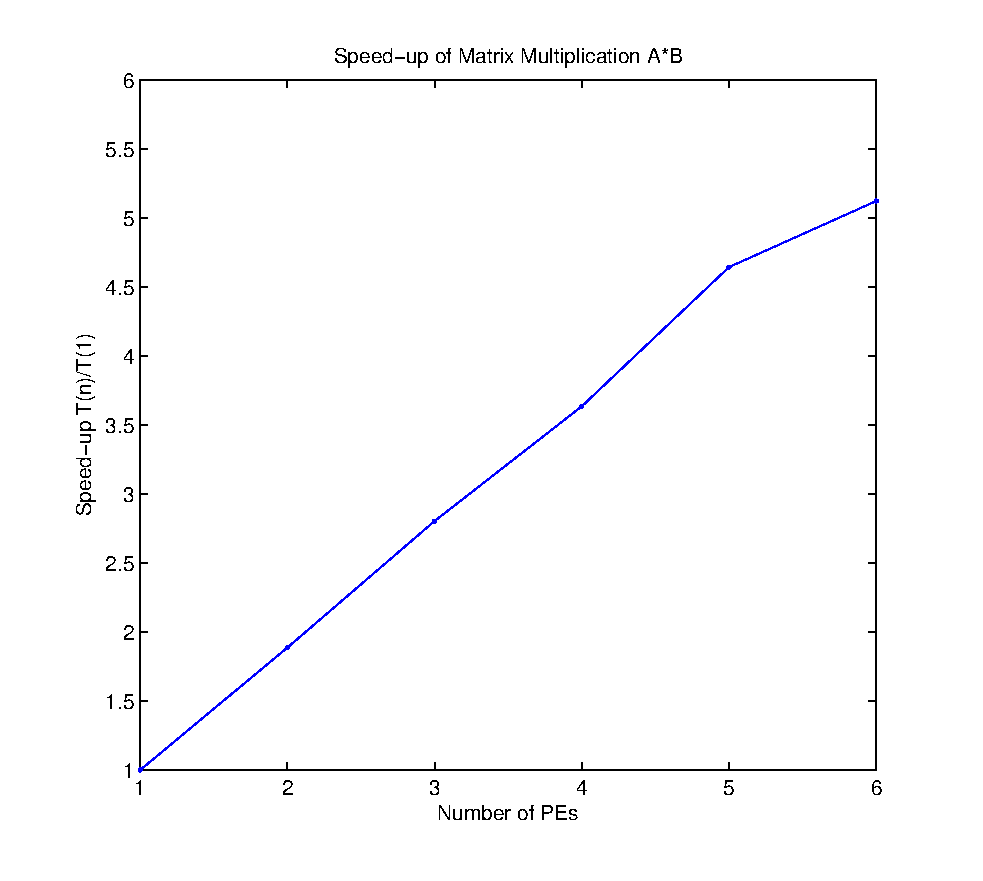
\includegraphics[width=4in]{speedup.eps}
	\caption{Speedup Plot}
	\label{fig:figure1}
	\end{center}
\end{figure}

\begin{figure}[htp]
	\begin{center}
	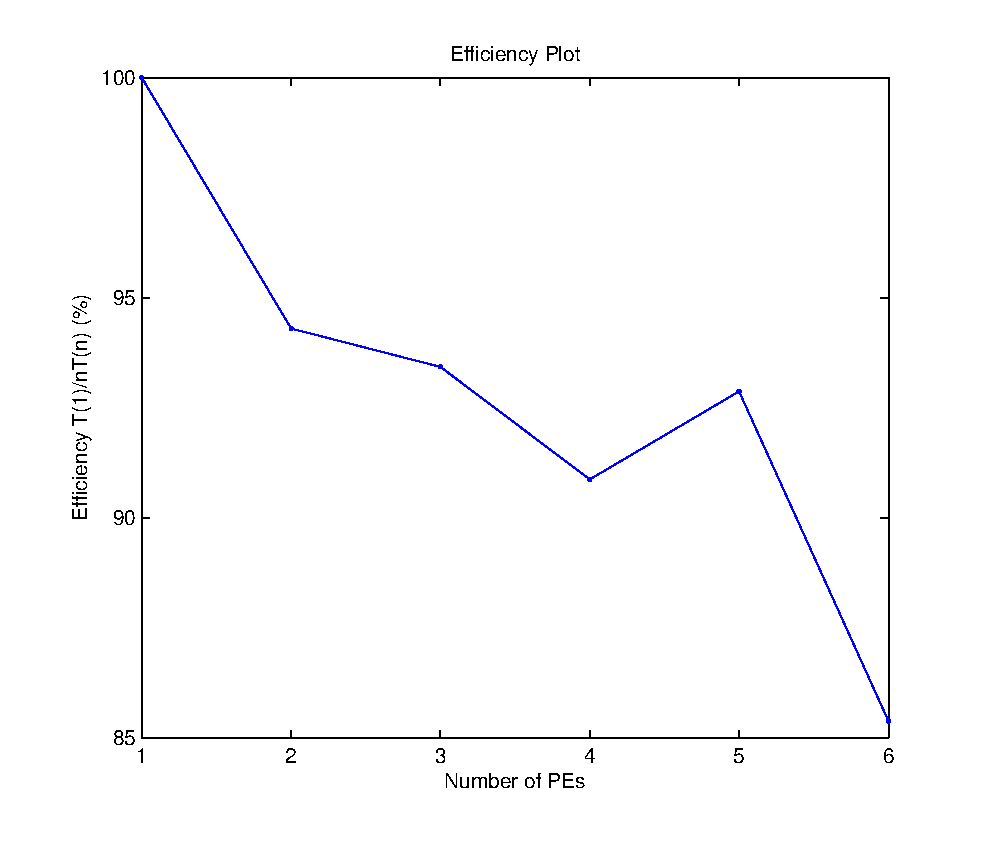
\includegraphics[width=4in]{efficiency.eps}
	\caption{Efficiency Plot}
	\label{fig:figure1}
	\end{center}
\end{figure}

\newpage
\section*{Appendix A - Sequential Operation}
\lstinputlisting{../H5-Sequential.c}

\newpage
\section*{Appendix B - Parallel Operation}
\lstinputlisting{../H5-Parallel.c}

\end{document}